\chapter{Analyse et Spécification des Besoins}
\label{chap:requirements_analysis}

\section{Introduction}

\par Ce chapitre se concentre sur l'analyse et la spécification des besoins de l'application \textbf{TuniPark}, après avoir introduit le contexte global du projet ainsi que la solution suggérée. Cette phase consiste à repérer les différents intervenants du système, de définir les fonctionnalités attendues ainsi que les contraintes techniques et qualitatives à respecter au cours du développement.

\par Dans un premier temps, ce chapitre introduit les intervenants dans le système. Il énonce ensuite les exigences fonctionnelles et non fonctionnelles de l'application avant de présenter les diagrammes UML majeurs employés pour la modélisation du système.
\section{Identification des acteurs}

\par L'application TuniPark fait intervenir deux principaux acteurs : l'utilisateur et l'administrateur. Chacun possède des responsabilités spécifiques au sein du système.

\subsection{Utilisateur}

\par L'utilisateur représente toute personne utilisant l'application mobile. Selon son besoin, il peut agir en tant que conducteur recherchant une place de stationnement ou en tant que propriétaire souhaitant proposer un parking privé. Il peut rechercher des parkings, effectuer un paiement, démarrer une session de stationnement, publier un parking privé, consulter son historique ainsi que gérer son profil.

\subsection{Administrateur}

\par L'administrateur interagit  l'interface web afin de superviser le fonctionnement de l'application. Il est chargé de consulter les demandes de création de parkings privés, d'approuver ou de rejeter les annonces, de gérer les parkings validés et de consulter les statistiques générales de la plateforme.

\section{Besoins fonctionnels}

\par Les besoins fonctionnels décrivent les services que doit fournir l'application TuniPark.

\par L'application doit permettre à l'utilisateur de :

\begin{itemize}
    \item créer un compte et s'authentifier ;
    \item se connecter avec Google ;
    \item réinitialiser son mot de passe ;
    \item rechercher des parkings à proximité ;
    \item consulter les parkings sur une carte interactive ;
    \item afficher les informations détaillées d'un parking ;
    \item sélectionner le nombre de places souhaitées ;
    \item effectuer un paiement sécurisé via Flouci ;
    \item démarrer automatiquement une session de stationnement après le paiement ;
    \item prolonger une session de stationnement ;
    \item consulter l'historique des sessions ;
    \item recevoir des notifications ;
    \item publier un parking privé ;
    \item ajouter des photos, les informations du parking ainsi qu'un document justificatif de propriété ;
    \item définir les tarifs et les horaires d'ouverture ;
    \item modifier ou archiver un parking publié ;
    \item consulter les revenus générés par ses parkings ;
    \item gérer son profil personnel.
\end{itemize}

\par L'application doit permettre à l'administrateur de :

\begin{itemize}
    \item s'authentifier de manière sécurisée ;
    \item consulter les demandes de création de parkings privés ;
    \item approuver ou rejeter les parkings proposés ;
    \item gérer les parkings validés ;
    \item consulter les revenus et les statistiques globales ;
    \item superviser le bon fonctionnement de la plateforme.
\end{itemize}
\section{Besoins non fonctionnels}

\par Les besoins non fonctionnels définissent les exigences de qualité que doit respecter l'application.

\begin{itemize}

\item \textbf{Sécurité :} Les données des utilisateurs doivent être protégées grâce à un mécanisme d'authentification sécurisé basé sur les JSON Web Tokens (JWT). Les sessions doivent être gérées de manière sécurisée à l'aide d'un Access Token et d'un Refresh Token. Les données sensibles stockées localement doivent être protégées et supprimées automatiquement lors de l'expiration de la session. Les paiements sont réalisés via la plateforme sécurisée Flouci.

\item \textbf{Performance :} L'accès rapide aux fonctionnalités telles que la recherche de places de parking, la visualisation de la carte, les suggestions et les actions de réservation et de paiement est essentiel pour garantir une expérience utilisateur sans accroc.

\item \textbf{Fiabilité :} Il est impératif que le système assure une disponibilité élevée des services et assure l'intégrité des données relatives aux utilisateurs, aux parkings, aux réservations et aux paiements.

\item \textbf{Utilisabilité :} L'interface web d'administration et L'application mobile doivent offrir une interface intuitive, ergonomique et facile à utiliser.

\item \textbf{Scalabilité :} L'architecture doit permettre l'ajout de nouveaux utilisateurs, de nouveaux parkings ainsi que de fonctionnalités émergentes sans dégrader les performances du système.

\item \textbf{Maintenabilité :} Le code source doit être organisé de manière modulaire et respecter une architecture claire afin de faciliter la maintenance, les corrections et l'évolution de la plateforme.

\item \textbf{Compatibilité :} L'application mobile faut être compatible avec les systèmes Android et iOS, tandis que l'interface d'administration doit être accessible depuis les navigateurs web récents les plus courants.

\end{itemize}
\section{Diagramme global des cas d'utilisation}

\par Le diagramme global des cas d'utilisation présente une vue d'ensemble des principales interactions entre les acteurs et l'application \textbf{TuniPark}. Il met en évidence les principales fonctionnalités offertes par le système ainsi que les services accessibles à chaque acteur.

\begin{figure}[H]
    \centering
    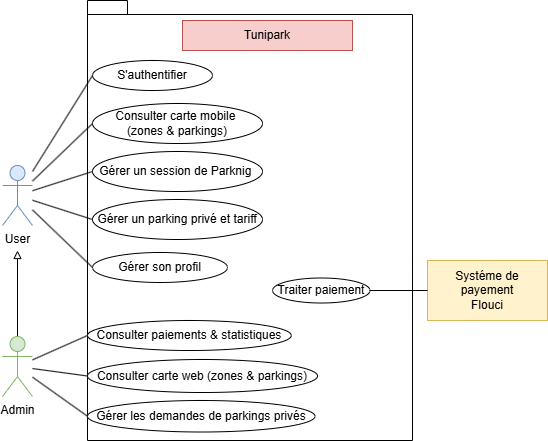
\includegraphics[width=0.95\textwidth]{img/useCase Diagram.png}
    \caption{Diagramme global des cas d'utilisation de l'application TuniPark}
    \label{fig:global_use_case}
\end{figure}

\par Comme l'illustre la Figure~\ref{fig:global_use_case}, l'utilisateur interagit avec l'application mobile afin de s'authentifier, consulter les parkings sur la carte, gérer ses sessions de stationnement, publier et administrer ses parkings privés ainsi que gérer son profil. Les opérations de paiement sont assurées par le service externe \textbf{Flouci}, intégré à l'application pour le traitement des transactions.

\par L'administrateur interagit l'interface web pour consulter la carte des parkings, gérer les demandes de création de parkings privés et accéder aux paiements ainsi qu'aux statistiques de la plateforme. Cette organisation permet de répartir clairement les responsabilités entre les différents acteurs tout en une gestion efficace du système.

\section{Description des principaux cas d'utilisation}

\par Cette section présente les principaux cas d'utilisation de l'application TuniPark. Les cas sélectionnés correspondent aux fonctionnalités essentielles proposées aux utilisateurs comme aux administrateurs, notamment la gestion des sessions de stationnement, la gestion des parkings privés, les paiements ainsi que l'administration de la plateforme.



\subsection{Authentification}

\begin{table}[H]
\centering
\renewcommand{\arraystretch}{1.25}
\begin{tabular}{|p{0.28\textwidth}|p{0.62\textwidth}|}
\hline
\textbf{Cas d'utilisation} &  Gérer l'authentification\\
\hline
\textbf{Rôle concerné} & Utilisateur, Administrateur \\
\hline
\textbf{Objectif} & Permettre à l'utilisateur ou à l'administrateur d'accéder à son espace personnel de manière sécurisée. \\
\hline
\textbf{Précondition} & L'utilisateur possède déjà un compte enregistré dans le système. \\
\hline
\textbf{Scénario principal} & L'utilisateur renseigne son adresse e-mail et son mot de passe. Le système vérifie les informations puis autorise l'accès à l'application selon le rôle de l'utilisateur. \\
\hline
\textbf{Exception} & Si les informations d'authentification sont incorrectes, Le système présente un message d'erreur et nie l'accès. \\
\hline
\textbf{Postcondition} & L'utilisateur est connecté et peut accéder aux fonctionnalités autorisées. \\
\hline
\end{tabular}
\caption{Authentification}
\label{tab:login}
\end{table}



\subsection{Gestion d'une session de parking}

\begin{table}[H]
\centering
\renewcommand{\arraystretch}{1.25}
\begin{tabular}{|p{0.28\textwidth}|p{0.62\textwidth}|}
\hline
\textbf{Cas d'utilisation} & Gérer une session de parking \\
\hline
\textbf{Rôle concerné} & Utilisateur \\
\hline
\textbf{Objectif} & Permettre à l'utilisateur de démarrer, consulter et arrêter une session de stationnement. \\
\hline
\textbf{Précondition} & L'utilisateur est authentifié et un parking est disponible. \\
\hline
\textbf{Scénario principal} & L'utilisateur sélectionne un parking, consulte ses informations, effectue le paiement puis le système démarre automatiquement la session de stationnement. \\
\hline
\textbf{Exception} & Si aucune place n'est disponible ou si une erreur survient, le système notifie l'utilisateur. \\
\hline
\textbf{Postcondition} & Une session de stationnement est créée et enregistrée. \\
\hline
\end{tabular}
\caption{Gestion d'une session de parking}
\label{tab:parking_session}
\end{table}




\subsection{Gestion d'un parking privé}

\begin{table}[H]
\centering
\renewcommand{\arraystretch}{1.25}
\begin{tabular}{|p{0.28\textwidth}|p{0.62\textwidth}|}
\hline
\textbf{Cas d'utilisation} & Gérer un parking privé \\
\hline
\textbf{Rôle concerné} & Utilisateur \\
\hline
\textbf{Objectif} & Permettre à un utilisateur de publier et gérer un parking privé ainsi que sa tarification. \\
\hline
\textbf{Précondition} & L'utilisateur est authentifié. \\
\hline
\textbf{Scénario principal} & L'utilisateur renseigne les informations du parking (adresse, nombre de places, disponibilité et tarif), puis soumet sa demande. Après validation par l'administrateur, le parking devient disponible sur la plateforme. \\
\hline
\textbf{Exception} & Si les informations sont incomplètes ou invalides, la demande est refusée jusqu'à correction. \\
\hline
\textbf{Postcondition} & Le parking est enregistré ou mis à jour dans le système. \\
\hline
\end{tabular}
\caption{Gestion d'un parking privé}
\label{tab:private_parking}
\end{table}

\subsection{Paiement d'une session}

\begin{table}[H]
\centering
\renewcommand{\arraystretch}{1.25}
\begin{tabular}{|p{0.28\textwidth}|p{0.62\textwidth}|}
\hline
\textbf{Cas d'utilisation} & Effectuer un paiement \\
\hline
\textbf{Rôle concerné} & Utilisateur \\
\hline
\textbf{Objectif} & Permettre à l'utilisateur de payer les frais de stationnement via le service Flouci. \\
\hline
\textbf{Précondition} & L'utilisateur a sélectionné un parking. \\
\hline
\textbf{Scénario principal} & Le système calcule le montant à payer selon les informations du parking. L'utilisateur est redirigé vers Flouci afin d'effectuer le paiement. Après validation de la transaction, la session de stationnement est créée automatiquement. \\
\hline
\textbf{Exception} & Si le paiement échoue ou est annulé, la transaction est marquée comme non effectuée et l'utilisateur est informé. \\
\hline
\textbf{Postcondition} & Le paiement est enregistré et la session de stationnement est démarrée. \\
\hline
\end{tabular}
\caption{Paiement d'une session}
\label{tab:payment}
\end{table}

\subsection{Validation des parkings privés}

\begin{table}[H]
\centering
\renewcommand{\arraystretch}{1.25}
\begin{tabular}{|p{0.28\textwidth}|p{0.62\textwidth}|}
\hline
\textbf{Cas d'utilisation} & Traiter les demandes de parkings privés \\
\hline
\textbf{Rôle concerné} & Administrateur \\
\hline
\textbf{Objectif} & Permettre à l'administrateur de valider ou refuser les requêtes de création de parkings privés. \\
\hline
\textbf{Précondition} & Une ou plusieurs demandes sont en attente de validation. \\
\hline
\textbf{Scénario principal} & L'administrateur consulte les demandes, vérifie les informations fournies puis accepte ou refuse la publication du parking. \\
\hline
\textbf{Exception} & Si les informations sont incomplètes ou incorrectes, la demande est rejetée avec un motif. \\
\hline
\textbf{Postcondition} & Le statut de la demande est mis à jour et l'utilisateur est informé de la décision. \\
\hline
\end{tabular}
\caption{Validation des parkings privés}
\label{tab:admin_private_parking}
\end{table}


\section{Product Backlog}

\par Ce dernier regroupe les principales fonctionnalités identifiées lors de l'analyse des besoins de l'application \textbf{TuniPark}. Il a servi de référence tout au long du développement afin de planifier les tâches, définir les priorités et organiser les différentes itérations du projet.

\par Les fonctionnalités ont été réparties selon plusieurs modules, notamment l'authentification, la gestion des parkings, les sessions de stationnement, les paiements, les notifications ainsi que l'administration de l'application.

\renewcommand{\arraystretch}{1.25}
\small

\begin{longtable}{|p{0.06\textwidth}|p{0.18\textwidth}|p{0.46\textwidth}|p{0.13\textwidth}|p{0.10\textwidth}|}
\caption{Product Backlog de l'application TuniPark}
\label{tab:product_backlog}\\

\hline
\textbf{ID} & \textbf{Module} & \textbf{User Story} & \textbf{Acteur} & \textbf{Priorité} \\
\hline
\endfirsthead

\hline
\textbf{ID} & \textbf{Module} & \textbf{User Story} & \textbf{Acteur} & \textbf{Priorité} \\
\hline
\endhead

1 & Authentification & En tant que personne utilisant l'application, mon désir est de constituer un compte pour avoir accès aux services proposés. & Utilisateur & Élevée \\
\hline

2 & Authentification & En tant qu'utilisateur, mon souhait est de me connecter en toute sécurité pour accéder à mon espace personnel. & Utilisateur / Admin & Élevée \\
\hline

3 & Authentification & Dans mon rôle d'utilisateur, je désire réinitialiser mon mot de passe via un code OTP reçu par e-mail ou téléphone. & Utilisateur & Élevée \\
\hline

4 & Carte & Dans mon rôle d'utilisateur, je désire visualiser les parkings disponibles sur une carte interactive afin de choisir celui qui me convient. & Utilisateur & Élevée \\
\hline

5 & Recherche & Dans mon rôle d'utilisateur, je désire rechercher un parking afin de trouver rapidement une place disponible. & Utilisateur & Élevée \\
\hline

6 & Session & Dans mon rôle d'utilisateur, je désire démarrer une session de stationnement après le paiement. & Utilisateur & Élevée \\
\hline

7 & Paiement & Dans mon rôle d'utilisateur, je désire payer ma session de stationnement via Flouci. & Utilisateur & Élevée \\
\hline

8 & Historique & Je souhaite, en tant qu'utilisateur, avoir la possibilité de consulter l'historique de mes sessions de stationnement. & Utilisateur & Moyenne \\
\hline

9 & Notifications & Dans mon rôle d'utilisateur, je désire recevoir des notifications concernant mes sessions et mes parkings. & Utilisateur & Moyenne \\
\hline

10 & Parking privé & Dans mon rôle d'utilisateur, je désire publier un parking privé afin de le proposer à la location. & Utilisateur & Élevée \\
\hline

11 & Parking privé & Dans mon rôle d'utilisateur, je désire ajouter des photos, une description, un tarif, des horaires et un document justificatif lors de la création d'un parking. & Utilisateur & Élevée \\
\hline

12 & Parking privé & Dans mon rôle d'utilisateur, je désire modifier ou archiver mes parkings. & Utilisateur & Moyenne \\
\hline

13 & Revenus & Dans mon rôle d'utilisateur, je désire consulter les revenus générés par mes parkings. & Utilisateur & Moyenne \\
\hline

14 & Administration & En tant qu'administrateur, je souhaite consulter les demandes de création de parkings privés. & Admin & Élevée \\
\hline

15 & Administration & En tant qu'administrateur, je souhaite approuver ou rejeter les parkings proposés. & Admin & Élevée \\
\hline

16 & Tableau de bord & En tant qu'administrateur, je souhaite consulter les statistiques générales de l'application. & Admin & Moyenne \\
\hline

17 & Revenus & En tant qu'administrateur, je souhaite consulter les revenus générés par la plateforme. & Admin & Moyenne \\
\hline

\end{longtable}

\normalsize

\par Ce Product Backlog a permis de structurer le développement de TuniPark en définissant les fonctionnalités à implémenter selon leur priorité. Les fonctionnalités critiques, notamment l'authentification, la gestion des parkings, les sessions de stationnement et les paiements, ont été développées en priorité. Les fonctionnalités complémentaires, comme les notifications, les statistiques et la gestion des revenus, ont ensuite été intégrées afin d'enrichir l'application et d'améliorer l'expérience utilisateur.

\section{Conclusion}

\par Ce chapitre a présenté l'analyse et la spécification des besoins de l'application \textbf{TuniPark}. Il a permis d'identifier les différents acteurs du système, de définir les besoins fonctionnels et non fonctionnels, ainsi que de présenter le diagramme global des cas d'utilisation.

\par Les principaux cas d'utilisation ont ensuite été décrits afin de mieux comprendre les interactions entre les utilisateurs, l'administrateur et l'application. Enfin, le Product Backlog a été établi pour organiser les fonctionnalités à développer et définir leurs priorités.

\par Le prochain chapitre portera sur la conception et à l'architecture de l'application. Il présentera l'architecture générale du système, les choix techniques adoptés, la modélisation de la base de données ainsi que les différents diagrammes UML utilisés lors de la conception.